% Seções 2.1, 2.4 e 2.5 do relatório parcial (INE5429): handshake do TLS 1.3,
% tamanho de chave como problema de rede e mini-exemplo.
% Compilar com pdflatex duas vezes.
\documentclass[12pt,a4paper]{article}
\usepackage[T1]{fontenc}
\usepackage[utf8]{inputenc}
\usepackage[brazil]{babel}
\usepackage{lmodern}
\usepackage[margin=2.5cm]{geometry}
\usepackage{setspace}
\usepackage{booktabs}
\usepackage{graphicx}
\usepackage{xcolor}
\usepackage{float}
\usepackage{amsmath}
\usepackage[labelsep=colon]{caption}
\usepackage{tikz}
\usetikzlibrary{arrows.meta,positioning,decorations.pathreplacing}
\usepackage{etoolbox}
\AtBeginEnvironment{tikzpicture}{\linespread{1}\selectfont}
\usepackage{url}
\usepackage[hidelinks]{hyperref}

\setstretch{1.5}
\setlength{\emergencystretch}{2em}
\definecolor{pq}{RGB}{217,98,43}
\definecolor{classico}{RGB}{61,90,128}
\definecolor{perda}{RGB}{179,38,30}
\newcommand{\todo}[1]{\textcolor{red}{\textbf{[#1]}}}
\newcommand{\fonte}[1]{\par\vspace{4pt}{\small Fonte: #1}}

\begin{document}


\setcounter{section}{1}
\section{Desenvolvimento}


\setcounter{subsection}{0}
\subsection{Handshake do TLS 1.3}

O TLS (Transport Layer Security) é o protocolo que protege a maior
parte das conexões na internet, como as do HTTPS, criando um canal seguro
sobre o TCP. Sua versão 1.3, hoje especificada pela RFC~9846 (RESCORLA,
2026), que substituiu a RFC~8446 (RESCORLA, 2018) em julho de 2026, é
dividida em duas partes: o handshake, em que cliente e servidor
combinam os parâmetros da conexão, se autenticam e estabelecem um segredo
compartilhado, e a camada de registro, que usa as chaves derivadas desse
segredo para cifrar os dados da aplicação.

Uma das principais mudanças do TLS~1.3 em relação às versões anteriores é
que o handshake completo leva apenas uma ida e volta (1-RTT) entre cliente
e servidor. Isso só é possível porque o cliente envia sua parte da troca de
chaves já na primeira mensagem, o \texttt{ClientHello}, sem esperar o
servidor dizer qual algoritmo prefere. Essa parte vai dentro de uma
extensão chamada \texttt{key\_share} (RESCORLA, 2026, seção 4.3.8), e é
justamente nela que a chave pós-quântica entra, como mostra a
Figura~\ref{fig:handshake}.

\begin{figure}[H]
\centering
\caption{Handshake completo do TLS 1.3, com o tamanho do \texttt{key\_share} na troca clássica (X25519) e na híbrida (X25519MLKEM768)}
\label{fig:handshake}
\begin{tikzpicture}[>=Stealth, font=\small]
  \node at (0,0) {Cliente};
  \node at (10,0) {Servidor};
  \draw[thick] (0,-0.3) -- (0,-8.4);
  \draw[thick] (10,-0.3) -- (10,-8.4);
  % ClientHello
  \node at (5,-0.75) {\texttt{ClientHello}};
  \draw[->, very thick, pq] (0,-1.1) -- (10,-1.4);
  \node[pq] at (5,-1.75) {\footnotesize \texttt{key\_share}: 32 bytes (clássico) $\rightarrow$ 1216 bytes (híbrido)};
  % ServerHello
  \node at (5,-2.6) {\texttt{ServerHello}};
  \draw[->, very thick, pq] (10,-2.95) -- (0,-3.25);
  \node[pq] at (5,-3.6) {\footnotesize \texttt{key\_share}: 32 bytes $\rightarrow$ 1120 bytes};
  % Flight cifrado
  \node[classico] at (5,-4.45) {\footnotesize \texttt{\{EncryptedExtensions, Certificate,}};
  \node[classico] at (5,-4.85) {\footnotesize \texttt{CertificateVerify, Finished\}}};
  \draw[->, classico] (10,-5.2) -- (0,-5.5);
  % Finished do cliente
  \node[classico] at (5,-6.4) {\footnotesize \texttt{\{Finished\}} + dados da aplicação};
  \draw[->, classico] (0,-6.75) -- (10,-7.05);
  \node[gray] at (5,-7.9) {\footnotesize \{\,\} = mensagens já cifradas com chaves derivadas da troca};
\end{tikzpicture}
\fonte{Adaptado de Rescorla (2026, Figura 1); tamanhos de Kwiatkowski et al. (2026, seções 4.1 e 4.2).}
\end{figure}

O servidor escolhe um dos algoritmos oferecidos pelo cliente e responde com
a sua própria parte da troca no \texttt{ServerHello}. A partir daí, os dois
lados calculam o mesmo segredo, que é usado para derivar as chaves da
sessão (RESCORLA, 2026, seção 7.1). Todas as mensagens seguintes já vão
cifradas: o servidor envia seu certificado, uma assinatura sobre o
handshake (\texttt{CertificateVerify}) e um código de autenticação de
mensagem (\texttt{Finished}), e o cliente responde com o seu próprio
\texttt{Finished}, já podendo enviar dados.

Como o cliente precisa adivinhar qual algoritmo o servidor vai aceitar, ele
pode errar. Nesse caso, o servidor responde com um
\texttt{HelloRetryRequest} (RESCORLA, 2026, seção 4.2.4) e o cliente
precisa recomeçar o handshake, o que custa uma ida e volta a mais. Para
evitar isso, o cliente pode enviar chaves de mais de um algoritmo no mesmo
\texttt{ClientHello}, mas isso deixa a mensagem maior (AHMAD; JAMAL;
KRIVIT, 2026). O OpenSSL~3.5, por exemplo, envia por padrão duas chaves:
uma híbrida pós-quântica e uma X25519 clássica (OPENSSL PROJECT, 2025).

Outro ponto importante é que, no TLS~1.3, o sigilo e a autenticação vêm de
lugares diferentes. O sigilo depende do segredo obtido na troca de chaves,
enquanto a autenticação depende da assinatura do \texttt{CertificateVerify}
e do \texttt{Finished} (RESCORLA, 2026, seções 4.5.2 e 4.5.3). Essa
separação faz diferença diante de um computador quântico, como mostra a
Figura~\ref{fig:hndl}: um atacante pode gravar o tráfego hoje e decifrá-lo
no futuro, quando conseguir quebrar a troca de chaves (harvest now,
decrypt later), mas, para falsificar a autenticação, ele precisaria do
computador quântico durante o próprio handshake. Por isso, a migração para
algoritmos pós-quânticos começou pela troca de chaves (ADRIAN et al.,
2024), e este trabalho também mantém os certificados clássicos, variando
apenas a troca.

\begin{figure}[H]
\centering
\caption{Por que a troca de chaves precisa migrar antes da autenticação}
\label{fig:hndl}
\begin{tikzpicture}[>=Stealth, font=\small]
  \draw[->, thick] (0,0) -- (12,0) node[right] {tempo};
  \fill[classico] (1.5,0) circle (4pt);
  \node[below=4pt] at (1.5,0) {hoje: handshake};
  \fill[perda] (10,0) circle (4pt);
  \node[below=6pt] at (10,0) {futuro: computador quântico};
  \draw[->, thick, dashed, pq] (1.5,0.3) to[bend left=25] (10,0.3);
  \node[pq] at (5.75,1.75) {troca de chaves: gravada hoje, decifrada no futuro};
  \node[classico, align=center] at (1.5,-1.6) {autenticação: só pode ser\\falsificada neste momento};
\end{tikzpicture}
\fonte{Elaborado pelos autores.}
\end{figure}

Para o TLS, cada algoritmo de troca de chaves é um ``grupo'' negociado. No
caso de um KEM, o \texttt{key\_share} do cliente leva a chave
de encapsulamento e o do servidor leva o ciphertext. A RFC~9954
descreve como combinar dois algoritmos numa troca híbrida (STEBILA;
FLUHRER; GUERON, 2026), e a RFC~10024 define o grupo
\texttt{X25519MLKEM768} (KWIATKOWSKI et al., 2026): o cliente envia sua
chave ML-KEM-768 seguida da sua chave X25519, o servidor responde com o
ciphertext seguido da sua chave X25519, e os dois segredos de
32~bytes são concatenados em um único segredo de 64~bytes. Esses tamanhos
são o ponto de partida do problema discutido na próxima seção.


\setcounter{subsection}{3}
\subsection{Tamanho de chave como problema de rede}
\label{sec:rede}

O ML-KEM é rápido de calcular, e por isso seu custo no TLS não está no
processamento, mas no tamanho das mensagens (RISTIC, 2026). Para entender
por que alguns bytes a mais viram atraso, é preciso olhar para como o
handshake é transportado pela rede.

\subsubsection*{Quanto cabe em um pacote}

Em uma rede Ethernet, cada pacote pode ter até 1500~bytes, valor chamado de
MTU (Maximum Transmission Unit). Desse total, 20~bytes vão para o
cabeçalho IP e 20~bytes para o cabeçalho TCP, sobrando 1460~bytes para os
dados, valor chamado de MSS (Maximum Segment Size), como mostra a
Figura~\ref{fig:encaps}. Quando a opção de timestamps do TCP está
ativa, ela ocupa mais 12~bytes e o MSS cai para 1448.

\begin{figure}[H]
\centering
\caption{Divisão de um pacote Ethernet de 1500 bytes (fora de escala)}
\label{fig:encaps}
\begin{tikzpicture}[font=\small]
  \draw (0,0) rectangle (1.6,0.9) node[midway, align=center] {IP\\20 B};
  \draw (1.6,0) rectangle (3.2,0.9) node[midway, align=center] {TCP\\20 B};
  \draw[fill=pq!15] (3.2,0) rectangle (13,0.9) node[midway, align=center] {dados do TLS (MSS)\\1460 B};
  \draw[decorate, decoration={brace, amplitude=6pt, mirror}] (0,-0.15) -- (13,-0.15) node[midway, below=8pt] {MTU = 1500 bytes};
\end{tikzpicture}
\fonte{Elaborado pelos autores.}
\end{figure}

Quando uma mensagem é maior que o MSS, o próprio TCP a divide em mais de um
segmento. Por isso, o termo mais correto aqui é \textit{segmentação}, e não
\textit{fragmentação}, que é o que acontece na camada IP e que o TCP
justamente tenta evitar respeitando o MSS.

\subsubsection*{De um para dois segmentos}

Com X25519, a chave do cliente tem só 32~bytes (LANGLEY; HAMBURG; TURNER,
2016), e o \texttt{ClientHello} inteiro cabe com folga em um segmento. Com
\texttt{X25519MLKEM768}, ela passa a ter 1216~bytes (KWIATKOWSKI et al.,
2026), o que sozinho ainda cabe, mas somado ao resto da mensagem pode
passar do limite, dependendo de quantas outras extensões o cliente envia. Ristic (2026) observou um \texttt{ClientHello} de 2117~bytes no
Chrome, que precisa então de dois segmentos (Figura~\ref{fig:barras}). A
equipe do Chrome relatou que essa divisão do \texttt{ClientHello} em dois
pacotes aumentou em 4\% a mediana da latência dos handshakes no Chrome para
desktop (ADRIAN et al., 2024).

\begin{figure}[H]
\centering
\caption{Tamanho do \texttt{key\_share} e do \texttt{ClientHello} em relação ao limite de um segmento}
\label{fig:barras}
\begin{tikzpicture}[font=\small, x=0.0045cm]
  % key_share X25519
  \node[left] at (0,2.4) {\texttt{key\_share} X25519};
  \fill[classico] (0,2.2) rectangle (32,2.6);
  \node[right] at (40,2.4) {32 B};
  % key_share híbrido
  \node[left] at (0,1.5) {\texttt{key\_share} híbrido};
  \fill[pq] (0,1.3) rectangle (1216,1.7);
  \node[right] at (1225,1.5) {1216 B};
  % ClientHello Chrome
  \node[left] at (0,0.6) {\texttt{ClientHello} (Chrome)};
  \fill[pq!55] (0,0.4) rectangle (2117,0.8);
  \node[right] at (2125,0.6) {2117 B};
  % MSS
  \draw[perda, thick, dashed] (1460,0.1) -- (1460,2.9);
  \node[perda, below] at (1460,0.1) {MSS = 1460 B (1 segmento)};
\end{tikzpicture}
\fonte{Elaborado pelos autores com dados de Langley, Hamburg e Turner (2016), Kwiatkowski et al. (2026) e Ristic (2026).}
\end{figure}

Essa divisão parece pequena, mas tem três consequências para o handshake.

\subsubsection*{1. Mais segmentos, mais chance de perda}
Se cada segmento é perdido de forma independente com probabilidade $p$
(que é justamente o modelo de perda do \texttt{tc netem}, usado no
experimento), a chance de perder pelo menos um entre $n$ segmentos é:
\begin{equation}
P(\text{perda}) = 1 - (1-p)^n
\end{equation}
Por exemplo, com 5\% de perda, a chance de algo dar errado no
\texttt{ClientHello} clássico (1 segmento) é de 5\%, mas no híbrido (2
segmentos) sobe para $1 - 0{,}95^2 = 9{,}75\%$, quase o dobro. A
Tabela~\ref{tab:perda} mostra o mesmo cálculo para as taxas de perda do
experimento.

\begin{table}[H]
\centering
\caption{Probabilidade de perder pelo menos um segmento de uma mensagem com $n$ segmentos}
\label{tab:perda}
\begin{tabular}{cccc}
\toprule
Perda por segmento ($p$) & $n=1$ & $n=2$ & $n=3$ \\
\midrule
1\%  & 1,00\%  & 1,99\%  & 2,97\% \\
5\%  & 5,00\%  & 9,75\%  & 14,26\% \\
10\% & 10,00\% & 19,00\% & 27,10\% \\
\bottomrule
\end{tabular}
\fonte{Elaborado pelos autores.}
\end{table}

\subsubsection*{2. Uma perda no handshake custa caro}
Em uma transferência longa, o TCP recupera uma perda rapidamente: os
segmentos que chegam depois do perdido fazem o receptor enviar ACKs
duplicados, e ao receber três deles o emissor retransmite o segmento
(ALLMAN; PAXSON; BLANTON, 2009, seção 3.2). No handshake, porém, cada lado
envia poucos segmentos e fica esperando a resposta, então, se o último
segmento se perde, não há nada depois dele para gerar esses ACKs
(Figura~\ref{fig:cauda}). Nesse caso, só um temporizador recupera a perda
(CHENG et al., 2021, seções 1.2 e 3.2): o RTO, cujo valor inicial
recomendado é de 1~segundo (PAXSON et al., 2011, seção 2.1), ou, em pilhas
mais modernas como a do Linux, a sonda TLP, que é enviada depois de cerca
de duas vezes o RTT (CHENG et al., 2021, seção 7.2).

\begin{figure}[H]
\centering
\caption{Recuperação de perda em uma transferência longa e no \texttt{ClientHello} híbrido}
\label{fig:cauda}
\begin{tikzpicture}[font=\small, seg/.style={draw, minimum width=1.1cm, minimum height=0.6cm}]
  \node[anchor=west] at (0,1.2) {(a) Transferência longa};
  \node[seg] at (0.6,0.4) {1};
  \node[seg] at (1.8,0.4) {2};
  \node[seg, fill=perda!70, text=white] at (3.0,0.4) {3 \texttt{x}};
  \node[seg] at (4.2,0.4) {4};
  \node[seg] at (5.4,0.4) {5};
  \node[seg] at (6.6,0.4) {6};
  \node[anchor=west, text=green!40!black, align=left] at (7.4,0.4) {4, 5 e 6 geram 3 ACKs duplicados:\\retransmissão em cerca de 1 RTT};
  \node[anchor=west] at (0,-0.9) {(b) \texttt{ClientHello} híbrido};
  \node[seg, minimum width=1.6cm, draw=pq] at (0.85,-1.7) {CH 1/2};
  \node[seg, minimum width=1.6cm, fill=perda!70, text=white] at (2.6,-1.7) {CH 2/2 \texttt{x}};
  \node[anchor=west, text=perda, align=left] at (3.6,-1.7) {nada chega depois, então não há ACKs duplicados:\\espera TLP ($\approx$ 2 RTT) ou RTO (1 s)};
\end{tikzpicture}
\fonte{Elaborado pelos autores com base em Allman, Paxson e Blanton (2009) e Cheng et al. (2021).}
\end{figure}

Para ter uma ideia do custo, considere uma rede com RTT de 50~ms. Sem
perdas, a aplicação começa a enviar dados depois de 2~RTTs, um para o
handshake do TCP e outro para o do TLS (KAMPANAKIS; CHILDS-KLEIN, 2024), ou
seja, cerca de 100~ms. Se o segundo segmento do \texttt{ClientHello} se
perde, a TLP acrescenta cerca de mais 100~ms, dobrando o tempo, e, se a
recuperação depender do RTO, o handshake passa de 1~segundo. Em uma
estimativa simplificada, multiplicando a chance de perda pelo custo da
TLP, com 5\% de perda o atraso médio extra seria de cerca de
$0{,}05 \times 100 = 5$~ms no \texttt{ClientHello} clássico e de
$0{,}0975 \times 100 \approx 9{,}8$~ms no híbrido. A média, porém, esconde
o principal efeito, que aparece nos casos piores: são poucas conexões que
perdem um segmento, mas cada uma delas fica muito mais lenta.

\subsubsection*{3. A janela inicial do TCP}
Logo depois de abrir a conexão, o TCP só pode enviar um número limitado de
segmentos antes de receber o primeiro ACK. A RFC~6928 recomenda uma janela
inicial de até 10~segmentos, limitada a 14\,600~bytes (CHU et al., 2013,
seção 2), ou seja, $10 \times 1460 = 14\,600$~bytes. Se a resposta do
servidor (do \texttt{ServerHello} até o \texttt{Finished}, incluindo os
certificados) passar desse valor, ele precisa esperar um ACK antes de
continuar, o que acrescenta um RTT inteiro (RISTIC, 2026). A chave
híbrida do servidor ocupa 1120~bytes, cerca de 7,7\% dessa janela, então
normalmente ainda cabe. Esse limite se torna o principal problema quando a
autenticação também migrar, já que assinaturas e chaves pós-quânticas nos
certificados são várias vezes maiores.

\subsubsection*{O problema na prática}

Embora o TLS sempre tenha permitido um \texttt{ClientHello} dividido em
mais de um segmento, muitos servidores e equipamentos de rede assumiam que
a mensagem chegaria inteira em uma única leitura. Com o
\texttt{ClientHello} pós-quântico, esse erro antigo passou a aparecer com
frequência: em vez de recusar o grupo desconhecido e usar o X25519, esses
servidores simplesmente derrubam a conexão (TLDR.FAIL, [s.d.]). A
Cloudflare relata que, em um estudo anterior, cerca de 0,34\% dos
servidores de origem examinados não completaram o handshake ao receber
primeiro uma chave pós-quântica (AHMAD; JAMAL; KRIVIT, 2026).

O efeito da perda de pacotes também já foi medido em ambiente controlado.
Paquin, Stebila e Tamvada (2020) usaram recursos de emulação de rede do
kernel Linux, como será feito neste trabalho, variando a perda de 0 a
20\%, e observaram que taxas acima de 3 a 5\% começam a ter impacto
significativo nos algoritmos pós-quânticos cujas mensagens ocupam muitos
pacotes. Já Kampanakis e Childs-Klein (2024) mostraram que, em redes
estáveis, o impacto no tempo total da conexão é menor do que no handshake e
diminui conforme mais dados são transferidos, mas que conexões em redes
com perda ou instáveis podem sofrer um impacto maior.

\subsubsection*{Hipótese}

A partir dessa análise, a hipótese a ser testada no experimento é que,
sem perda, a diferença entre X25519 e \texttt{X25519MLKEM768} deve ser
pequena, já que o custo está em bytes e não em idas e voltas. Conforme a
perda aumenta, o \texttt{ClientHello} em dois segmentos deve aumentar a
chance de uma perda no handshake e, com ela, os casos mais lentos da
distribuição, por causa das recuperações por temporizador. Por isso, além
da média, o experimento também deve observar a mediana e os percentis mais
altos (como o p95).


\subsection{Mini-exemplo}
\label{sec:mini}

Neste mini-exemplo, a entrada é o grupo negociado no handshake e a saída
é o tamanho das mensagens e o número de segmentos que elas ocupam na rede.
Primeiro, a Tabela~\ref{tab:tamanhos} mostra os tamanhos esperados, de
acordo com as especificações.

\begin{table}[H]
\centering
\caption{Tamanho do \texttt{key\_share} de cada lado, em bytes}
\label{tab:tamanhos}
\begin{tabular}{lccl}
\toprule
Grupo & Cliente & Servidor & Composição \\
\midrule
X25519 & 32 & 32 & chave pública X25519 \\
ML-KEM-768 (puro) & 1184 & 1088 & chave de encapsulamento / ciphertext \\
X25519MLKEM768 & 1216 & 1120 & parte ML-KEM + parte X25519 \\
\bottomrule
\end{tabular}
\fonte{Langley, Hamburg e Turner (2016), NIST (2024) e Kwiatkowski et al. (2026).}
\end{table}

Ou seja, trocar o X25519 pelo híbrido acrescenta $1216 - 32 = 1184$~bytes
ao \texttt{ClientHello} e $1120 - 32 = 1088$~bytes ao \texttt{ServerHello}.
Comparando com o MSS de 1460~bytes, só o \texttt{key\_share} híbrido já
ocupa $1216 / 1460 \approx 83\%$ de um segmento, sobrando cerca de
244~bytes para todo o resto do \texttt{ClientHello}, que também carrega
versão, números aleatórios, lista de cifras e outras extensões.

Para confirmar isso na prática, foram capturados handshakes TLS~1.3 entre
um cliente e um servidor OpenSSL~3.5, que já suporta ML-KEM sem precisar
de bibliotecas externas (OPENSSL PROJECT, 2025), rodando em dois
containers ligados por uma rede com MTU de 1500~bytes. O servidor usa um
certificado ECDSA clássico, já que só a troca de chaves varia. Como o
OpenSSL~3.5 envia por padrão as chaves híbrida e X25519 juntas, o grupo
foi fixado à mão em cada captura, para que as configurações não se
misturassem, e o padrão foi capturado à parte. A Tabela~\ref{tab:captura}
resume o que foi observado no Wireshark.

\begin{table}[H]
\centering
\caption{Resultados da captura (um handshake por configuração), em bytes entregues ao TCP, incluindo o cabeçalho de 5 bytes do registro TLS}
\label{tab:captura}
\footnotesize
\begin{tabular}{lcccc}
\toprule
Configuração & \texttt{ClientHello} & Segmentos & \texttt{ServerHello} & Resposta do servidor \\
 & (bytes) & do CH & (bytes) & (bytes / segmentos) \\
\midrule
X25519 & 217 & 1 & 127 & 764 / 1 \\
X25519MLKEM768 & 1393 & 1 & 1215 & 1842 / 2 \\
MLKEM768 & 1361 & 1 & 1183 & 1821 / 2 \\
Padrão OpenSSL (2 chaves) & 1451 & 2 & 1215 & 1841 / 2 \\
\bottomrule
\end{tabular}
\fonte{Elaborado pelos autores.}
\end{table}

O primeiro resultado é que os \texttt{key\_share} medidos batem exatamente
com a Tabela~\ref{tab:tamanhos}: 32 e 32~bytes no X25519, 1216 e
1120~bytes no híbrido e 1184 e 1088~bytes no ML-KEM-768 puro. O segundo
é menos óbvio: com o grupo híbrido sozinho, o \texttt{ClientHello} do
OpenSSL tem 1393~bytes e ainda cabe em um segmento. Ele é bem mais enxuto
que o do Chrome (2117~bytes), que carrega mais extensões. Quem passa para
dois segmentos é o padrão do OpenSSL, que envia as duas chaves. A segunda
entrada do \texttt{key\_share} acrescenta 36~bytes (32 da chave e 4 de
cabeçalho), a lista de grupos suportados acrescenta mais 14, e outras
pequenas diferenças completam os 58~bytes a mais em relação ao híbrido
sozinho. Isso leva a mensagem a 1451~bytes.

Esses 1451~bytes ficam abaixo dos 1460 do MSS calculado na
Seção~\ref{sec:rede}, e mesmo assim a mensagem foi dividida. Isso acontece
porque o Linux ativa os timestamps do TCP por padrão: o SYN anuncia um MSS
de 1460, mas cada segmento perde 12~bytes para a opção de timestamps,
sobrando 1448. O \texttt{ClientHello} foi então enviado como um segmento
de 1448~bytes seguido de outro com apenas 3, o que mostra como o limite é
estreito: com o híbrido sozinho, sobravam só 55~bytes. A
Figura~\ref{fig:captura} mostra esse caso no Wireshark.

\begin{figure}[H]
\centering
\caption{\texttt{ClientHello} do padrão do OpenSSL~3.5 (\texttt{X25519MLKEM768} + X25519) capturado no Wireshark}
\label{fig:captura}
% Print do Wireshark de captura/capturas/padrao-openssl.pcap (filtro tls.handshake.type == 1),
% mostrando "2 Reassembled TCP Segments (1451 bytes): #4(1448), #5(3)" e as duas
% entradas do key_share (1216 e 32 bytes). Salvar como captura-clienthello.png e
% trocar o \fbox abaixo por: 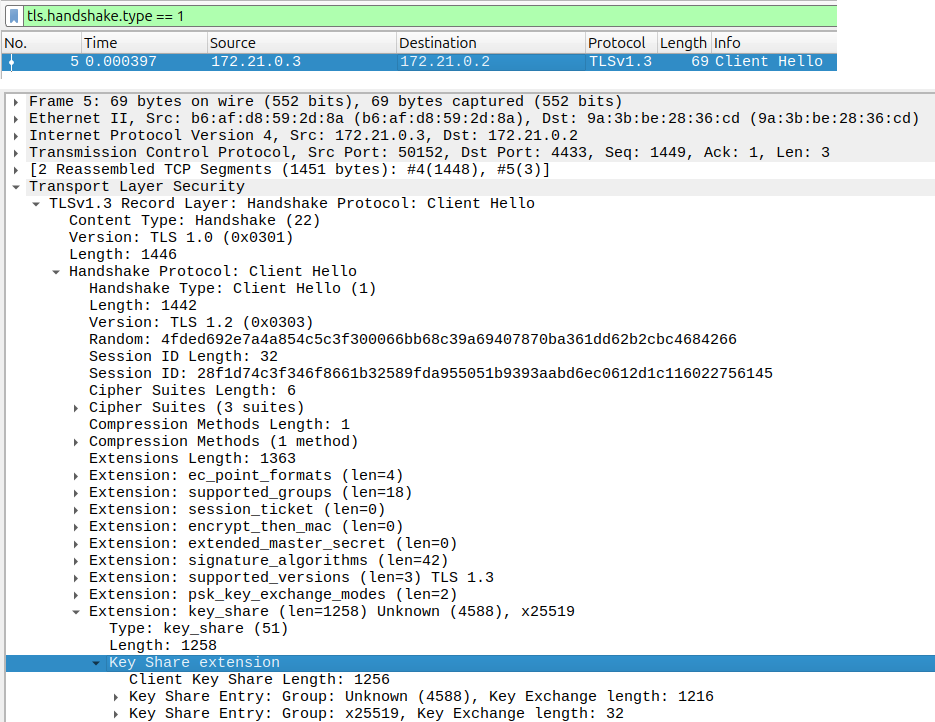
\includegraphics[width=\linewidth]{captura-clienthello.png}
\fbox{\parbox[c][5cm][c]{0.9\linewidth}{\centering \todo{colar imagem wireshark}}}
\fonte{Elaborado pelos autores.}
\end{figure}

Do lado do servidor, a resposta (do \texttt{ServerHello} ao
\texttt{Finished}) passou de 764~bytes em um segmento no X25519 para cerca
de 1840~bytes em dois segmentos nos grupos pós-quânticos. Ou seja, a
resposta do servidor também cruzou o limite de um segmento, inclusive no
híbrido sozinho. Mesmo assim, ela ocupa só cerca de 12,6\% da janela
inicial de 14\,600~bytes e não precisa esperar nenhum ACK. Como os
certificados continuam clássicos, a janela inicial ainda não é um
problema, como previsto na Seção~\ref{sec:rede}.

Esse resultado liga a teoria ao experimento. A passagem de um para dois
segmentos é exatamente a mudança que os testes vão combinar com
diferentes taxas de perda. Mas ela não acontece no mesmo lugar em todas as
configurações: com o grupo híbrido fixado, só a resposta do servidor é
dividida, enquanto no padrão do OpenSSL o \texttt{ClientHello} também é.
Por isso, o experimento deve incluir as duas configurações para observar
os dois efeitos separadamente.


% REFERÊNCIAS
\section*{Referências}
\begingroup
\setstretch{1.0}
\setlength{\parindent}{0pt}
\setlength{\parskip}{0.8em}
\newcommand{\refitem}[1]{\hangindent=1.5em #1\par}

\refitem{ADRIAN, D.; BECK, B.; BENJAMIN, D.; O'BRIEN, D. \textbf{Advancing
our amazing bet on asymmetric cryptography}. Google Blog, 23 maio 2024.
Disponível em:
\url{https://blog.google/chromium/advancing-our-amazing-bet-on-asymmetric/}.
Acesso em: 15 nov. 2026.}

\refitem{AHMAD, S.; JAMAL, Y.; KRIVIT, A. \textbf{Automatic Key Exchange}:
faster, post-quantum secure origin handshakes for 45 billion daily
connections (and counting). The Cloudflare Blog, 8 set. 2026. Disponível
em: \url{https://blog.cloudflare.com/automatic-key-exchange-for-origins/}.
Acesso em: 15 nov. 2026.}

\refitem{ALLMAN, M.; PAXSON, V.; BLANTON, E. \textbf{TCP congestion
control}. RFC 5681. Internet Engineering Task Force, set. 2009. Disponível
em: \url{https://www.rfc-editor.org/info/rfc5681}. Acesso em: 15 nov.
2026.}

\refitem{CHENG, Y.; CARDWELL, N.; DUKKIPATI, N.; JHA, P. \textbf{The
RACK-TLP loss detection algorithm for TCP}. RFC 8985. Internet Engineering
Task Force, fev. 2021. Disponível em:
\url{https://www.rfc-editor.org/info/rfc8985}. Acesso em: 15 nov. 2026.}

\refitem{CHU, J.; DUKKIPATI, N.; CHENG, Y.; MATHIS, M. \textbf{Increasing
TCP's initial window}. RFC 6928. Internet Engineering Task Force, abr.
2013. Disponível em: \url{https://www.rfc-editor.org/info/rfc6928}. Acesso
em: 15 nov. 2026.}

\refitem{KAMPANAKIS, P.; CHILDS-KLEIN, W. The impact of data-heavy,
post-quantum TLS 1.3 on the Time-To-Last-Byte of real-world connections.
In: WORKSHOP ON MEASUREMENTS, ATTACKS, AND DEFENSES FOR THE WEB (MADWeb),
2024, San Diego. \textbf{Proceedings} [...]. Reston: Internet Society,
2024. DOI: 10.14722/madweb.2024.23010.}

\refitem{KWIATKOWSKI, K.; KAMPANAKIS, P.; WESTERBAAN, B. E.; STEBILA, D.
\textbf{Post-quantum traditional (PQ/T) hybrid key agreement mechanisms for
TLS 1.3}. RFC 10024. Internet Engineering Task Force, ago. 2026.
Disponível em: \url{https://www.rfc-editor.org/info/rfc10024}. Acesso em:
15 nov. 2026.}

\refitem{LANGLEY, A.; HAMBURG, M.; TURNER, S. \textbf{Elliptic curves for
security}. RFC 7748. Internet Research Task Force, jan. 2016. Disponível
em: \url{https://www.rfc-editor.org/info/rfc7748}. Acesso em: 15 nov.
2026.}

\refitem{NATIONAL INSTITUTE OF STANDARDS AND TECHNOLOGY (NIST).
\textbf{Module-lattice-based key-encapsulation mechanism standard}. FIPS
203. Gaithersburg: NIST, ago. 2024. DOI: 10.6028/NIST.FIPS.203.}

\refitem{OPENSSL PROJECT. \textbf{OpenSSL 3.5 series release notes}. 2025.
Disponível em: \url{https://openssl-library.org/news/openssl-3.5-notes}.
Acesso em: 15 nov. 2026.}

\refitem{PAQUIN, C.; STEBILA, D.; TAMVADA, G. Benchmarking post-quantum
cryptography in TLS. In: DING, J.; TILLICH, J.-P. (ed.).
\textbf{Post-Quantum Cryptography}: PQCrypto 2020. Cham: Springer, 2020.
p. 72--91. (Lecture Notes in Computer Science, v. 12100).}

\refitem{PAXSON, V.; ALLMAN, M.; CHU, J.; SARGENT, M. \textbf{Computing
TCP's retransmission timer}. RFC 6298. Internet Engineering Task Force,
jun. 2011. Disponível em: \url{https://www.rfc-editor.org/info/rfc6298}.
Acesso em: 15 nov. 2026.}

\refitem{RESCORLA, E. \textbf{The Transport Layer Security (TLS) protocol
version 1.3}. RFC 8446. Internet Engineering Task Force, ago. 2018.
Disponível em: \url{https://www.rfc-editor.org/info/rfc8446}. Acesso em:
15 nov. 2026.}

\refitem{RESCORLA, E. \textbf{The Transport Layer Security (TLS) protocol
version 1.3}. RFC 9846. Internet Engineering Task Force, jul. 2026.
Disponível em: \url{https://www.rfc-editor.org/info/rfc9846}. Acesso em:
15 nov. 2026.}

\refitem{RISTIC, I. \textbf{Effect of post-quantum algorithms on networking
performance}. Red Sift Blog, 24 ago. 2026. Disponível em:
\url{https://redsift.com/blog/post-quantum-networking-performance}. Acesso
em: 15 nov. 2026.}

\refitem{STEBILA, D.; FLUHRER, S.; GUERON, S. \textbf{Hybrid key exchange
in TLS 1.3}. RFC 9954. Internet Engineering Task Force, jul. 2026.
Disponível em: \url{https://www.rfc-editor.org/info/rfc9954}. Acesso em:
15 nov. 2026.}

\refitem{TLDR.FAIL. \textbf{tldr.fail}. [s.d.]. Disponível em:
\url{https://tldr.fail/}. Acesso em: 15 nov. 2026.}
\endgroup


\end{document}
